\scanpage{19}
\uline{Definition of $\beta$}\qquad We define
\[
\beta(\Pi,\widetilde\Pi,p,\mathcal G,a)=(\unsure{\mathcal E|\Sigma},\mathcal G,\pi,\mathfrak Z)\quad\text{as follows :}
\]
$\unsure{\mathcal E|\Sigma}=$ group of pairs $(g,\bar g)$, with $g\in\mathcal G$, $\bar g\in\operatorname{Aut}(\widetilde\Pi)$ compatible with $g$
\[
\pi=\operatorname{Aut}(\widetilde\Pi/\Pi)
\]
$\unsure{\mathcal E|\Sigma}\longrightarrow\mathcal G$ by $(g,\bar g)\longmapsto g$, whence
\diagram{\begin{tikzcd}[ampersand replacement=\&]
1 \arrow[r,dash] \& \pi \arrow[r] \& \unsure{\mathcal E|\Sigma} \arrow[r,dash] \& \mathcal G \arrow[r] \& 1
\end{tikzcd}}
$\mathfrak Z=\operatorname{Ob}\widetilde\Pi$, with obvious action of $\unsure{\mathcal E|\Sigma}$ on $\mathfrak Z$\begin{tikzpicture}[baseline=0pt,x=1cm,y=1cm]
\fill (0.08,0) circle (0.018);
\fill (0.26,0.02) circle (0.018);
\draw[draw=black!60,line width=0.35pt,line cap=round] (0.43,0.06) -- (0.55,0.10);
\draw[draw=black!60,line width=0.35pt,line cap=round] (0.70,0.13) -- (0.86,0.17);
\end{tikzpicture}

Profinite variants\ldots

\textcircled{8} Consider, with notation \deleted{\unsure{of|of}} \S 7,
\[
\left(\diagram{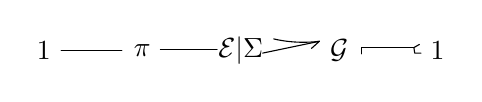
\begin{tikzpicture}[baseline=(extension.base),x=1cm,y=1cm,line cap=round,line join=round]
\node (oneleft) at (0,0) {$1$};
\node (kernel) at (1.25,0) {$\pi$};
\node (extension) at (2.50,0) {$\unsure{\mathcal E|\Sigma}$};
\node (quotient) at (3.75,0) {$\mathcal G$};
\node (oneright) at (5,0) {$1$};
\draw (0.22,0) -- (0.99,0);
\draw (1.48,0.01) -- (2.20,0.01);
\draw (2.78,-0.03) -- (3.50,0.12);
\draw (2.92,0.15) .. controls (3.13,0.10) and (3.35,0.10) .. (3.50,0.12) -- (3.40,0.03);
\draw (4.03,-0.04) -- (4.03,0.04) -- (4.70,0.04);
\draw (4.70,0.04) -- (4.77,0.08);
\draw (4.70,0.04) -- (4.71,-0.03) -- (4.79,-0.03);
\end{tikzpicture}}
\quad\text{and }\mathfrak Z\quad\unsure{\mathcal E|\Sigma}\text{-set}\ne\varnothing\text{ on which }\pi\text{ acts freely}\right)
\]
$\longleftrightarrow(\Pi,\widetilde\Pi,p,\mathcal G,a)$. We are going to interpret the datum of a triple $(\inserted{\chi,}\unsure{\tau|\mathcal T},T,\Phi)$, \inserted{$\chi:$} where $\unsure{\tau|\mathcal T}$ is an $\unsure{\mathcal E|\Sigma}$-set, $T$ a group $(\simeq\widehat{\mathbf Z}\;?)$, \inserted{$\chi:\mathcal G\longrightarrow\operatorname{Aut}(T)$ \unsure{$(\simeq\widehat{\mathbf Z}^{*}\unsure{)|?}\;\text{canonically}?)$}} and
\diagram{\begin{tikzcd}[ampersand replacement=\&]
\Phi:\unsure{\tau|\mathcal T} \arrow[r] \& \operatorname{Hom}_{\mathrm{gr}}(T,\pi)
\end{tikzcd}}
compatible with action of $\unsure{\mathcal E|\Sigma}$ (acting
\mspage{18}
